\section{Grafo}
\begin{definicion}
\label{"grafo conexo"}
Un grafo es un par ordenado $G=(V,E)$,donde:
\begin{itemize}
\item $V$ es un conjunto de vértices o nodos ($n=|V_G|$)
\item $E$ es un conjunto de aristas o arcos, que relacionan estos nodos
($m=|E_G|$)
\end{itemize}
\begin{figure}
  \centering
      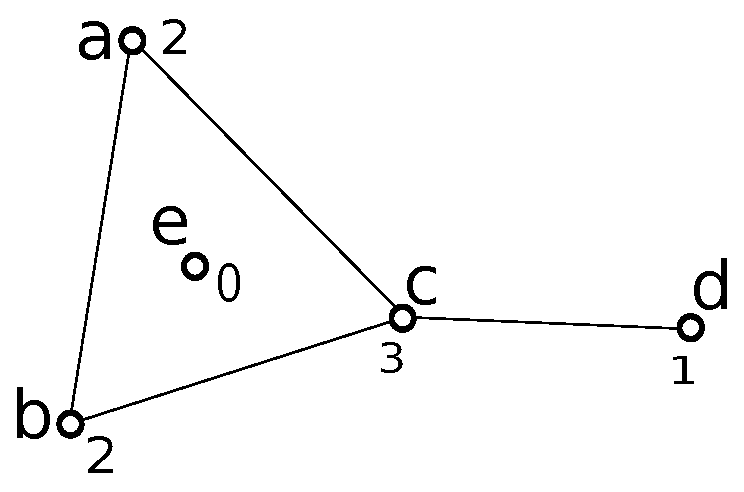
\includegraphics[width=0.5\textwidth]{imagen/grafo1}
  \caption{Grafo Dirigido}
  \label{fig:grafo1}
\end{figure}

Ejemplo (Figura \ref{fig:grafo1}):\\
$V=\{a,b,c,d,e\}$\\
$E=\{\{a,b\},\{b,c\},\{a,c\},\{c,d\}\}$, hacemos la simplifiación:  $E=\{ab,bc,ac,cd\}$ \\
\end{definicion}
En este material, no se considerarán los siguientes grafos:
\begin{enumerate}
\item $\{\{a,b\},\{b,a\}\}$ (Figura \ref{fig:ab})
\begin{figure}
  \centering
    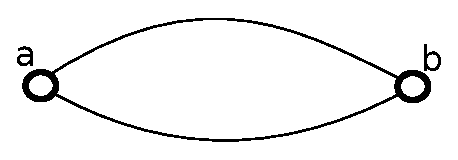
\includegraphics[width=0.5\textwidth]{imagen/grafoabab}
  \caption{Grafo ab}
  \label{fig:ab}
\end{figure}

\item $\{\{a,a\}\}$ (Figura \ref{fig:aa})
\begin{figure}
  \centering
    \includegraphics[width=0.25\textwidth]{imagen/grafoaa}
  \caption{Grafo aa}
  \label{fig:aa}
\end{figure}
\end{enumerate}
\begin{definicion}
Grado de un vértice $(d)$ \\
$d(v):$ número de vértices adyacentes al vértice $v$
\begin{enumerate}
\item Grado mínimo: $\delta(G)=0$
\item Grado máximo: $\Delta(G)=3$
\end{enumerate}
\end{definicion}
\subsection{Representación matricial}
\begin{enumerate}
\item Matriz de Incidencia

%Matriz de incidencia

\item Matriz de Adyacencia

%Matrix de adyacencia

\end{enumerate}
\subsection{Grafos Importantes}
\begin{enumerate}
\item {\bf Regular:} Cuando $\delta(G)=\Delta(G)$
\item {\bf Completo:} Donde $E_G=V_G^{(2)}$ \\
siendo: $V_G^{(2)}=\{uv|u,v \in V_G\}$ \\
\notacion $K_n$ es un grafo completo de $n$ vértices.
$$E_{K_n}=\frac{n(n-1)}{2}$$
%\begin{itemize}
%\item $n=1$
%\item $n=2$
%\item $n=3$
%\item $n=4$
%\item $n=5$ 

%Grafica de grafos completos

%\end{itemize}
\item {\bf Bipartido:}
Es un grafo $G=(U\cup W,E)$, donde $U\cap W=\phi$\\
y $E\subseteq \{uv|u\in U, v\in W\}$. Entonces: $0\leq m(G)\leq|U||W|$.

%Grafico de grafo bipartido
\begin{itemize}
\item {\bf Bipartido Completo:}
Cuando $m(G)=q.p$ donde $q=|U|$ y $p=|W|$.\\
\notacion $K_{p,q}$
%Grafico de grafo bipar completo

\item {\bf Estrella:}
Es el grafo $K_{1,q}$

%Grafico de grafo estrella
\end{itemize}

\item {\bf Grafo de las Aristas:}
Es el grafo que se toma al considerar las aristas como nodos y se traza una arista entre ellas si tienen un vértice en común en el grafo original.

%Grafico

\end{enumerate}
\begin{teorema}
\label{teoconex}
En un grafo $G$, la suma de los grados de todos los vértices es igual
al doble del número de aristas.
$$\sum_{v\in {V_G}}^n{d(v)} = {2|E_G|}$$
\end{teorema}
\begin{proof}
Por inducción en $|E_G|$ \\
Base: $|E_G|=0$
$$\sum_{v\in {V_G}}^n{d(v)} = \sum_{v\in {V_G}}^n0 = 0 = 2|E_G|$$
Paso de inducción $|E_G|>0$ , escoja $uv \in E_G$, defina: 
$$H=(V_G,E_G-\{uv\})$$
Por hipótesis inductiva:
$$\sum_{v\in {V_H}}^n{d(v)} = 2|E_H| = 2(|E_G|-1) = 2|E_G|-2$$
Paso:
$$\sum_{v\in {V_G}}^n{d(v)} = \sum_{v\in {V_H}}^n{d(v)}+2 = |E_G|-2+2 = 2|E_G|$$
\end{proof}

\begin{teorema}
Todo grafo tiene un número par de vértices de grado impar.
\end{teorema}
\begin{proof}
Por contradicción, suponga que existe un número impar de vertices de grado impar.\\
Entonces: \\
$$\sum_{v\in {V_G}}^n{d(v)} = \sum_{v\in {V_G}\ | d(v)\ es\ par}{d(v)}+\sum_{v\in {V_G}\ | d(v)\ es\ impar}{d(v)}$$
$$\sum_{v\in {V_G}}^n{d(v)} = Par + Impar =Impar$$
Contradición:
$$\sum_{v\in {V_G}}^n{d(v)} = 2|E_G|$$
\end{proof}
\begin{teorema}
En un grafo $G$ existe por lo menos dos vértices con el mismo grado.
\end{teorema}
\begin{proof}
Sea $V=\{1,2,3,...n\}$, entonces: $0\leq d(v)\leq n-1$

Suponga que todos los vértices tienen grados distintos, entonces existe un vertice de grado $0$ y un vértice de grado $n-1$.
%Grafico de vertice de grado n-1 con vertice grado 0

Contradición: El vértice de grado $n-1$ tendría que estar unido al vertice de grado $0$.
\end{proof}
\subsection{Unión, Intersección y Subgrafo}
\begin{itemize}
\item {\bf Unión:}
$$G \cup H = (V_G \cup V_H, E_G \cup E_H)$$
\item {\bf Intersección:}
$$G \cap H = (V_G \cap V_H, E_G \cap E_H)$$
\item {\bf Subgrafo:} $G$ es un subgrafo de $H$, si $V_G \subseteq V_H$ y
$V_H \subseteq E_H$
\end{itemize}

\subsection{Caminos}

%Grafico de camino
Es una sucesión finita en la que aparecen vértices y aristas alternadamente.
No es camino si se repiten vértices. Se define como la longitud de un camino al número de aristas del mismo.

\subsubsection{Camino máximo}
Un camino $C$ de $G$ es máximo si no existe un camino $C'$ tal que $|C|<|C'|$.
\subsubsection{Camino maximal}
Un camino $C$ es maximal si no existe $C'$ tal que $C\subset C'$.

%Grafica de camino maximo y maximal

\begin{teorema}
Para todo grafo $G$ tal que $d(v)\geq k\ \forall V\in V_G$, existe un camino de longitud mayor o igual a $k$.\\
\end{teorema}
\begin{proof}
Tome camino maximal, sea $v$ un extremo de este camino, como $d(v)\geq k$ y $C$ es maximal, entonces $v$ es adyacente a por lo menos $k$ vértices del camino y por tanto $|C|\geq k$.

%Grafico de demostracion

\end{proof}
\subsection{Circuito}
Es un camino cerrado, donde los únicos vértices que se repetidos son el primero y el último.
%Grafico de circuito

\begin{teorema}
Si $\delta(G)\geq2$, entonces $G$ tiene circuito.
\end{teorema}
\begin{proof}
Tome un camino maximal $C$. Sea $v$ un extremo de este camino,
como $d(v)\geq2$ y $C$ es un maximal, existe $u\neq v$, tal que $uv\in E_G$ y por tanto un circuito $C'$.
%por definir 
\end{proof}

\section{Cortes}
Dado un conjunto $X\subset V_G$, decimos que $\partial (X)=\{uv /u\in x, v\in V_G \setminus x \}$ es el corte asociado a $x$.

%Grafico de corte

Si $x=V_G$, entoces $\partial (x)=\phi$.

%Grafico de corte2

\begin{definicion}
Una arista $a$ es un ``puente'', si $\{a\}$ es un corte.

%Definir mejor
%Graficar puente
\end{definicion}
\begin{teorema}
Si todos los vértices del grafo $G$ tiene grado par, entonces $G$ no tiene puentes.
\end{teorema}
\begin{proof}
Asumimos que existe un puente $a$, sea $H=(V_G,E_G-\{a\})$.
Sea $H_1$ y $H_2$ los componentes de $H$. En $H_1$ existe
un solo vértice de grado impar. Contradicción por que :
$$\sum_{v\in {V_{H_1}}}^n{d(v)}=2|E_H|$$

%Grafico de demostracion

\end{proof}
\begin{teorema}
En todo grafo $G$ tal que $|V_G|\geq 2$, existe $X\subseteq V_G$ tal que $\partial (X)\geq\frac1{2}|E_G|$.

\end{teorema}

